\documentclass{article}
\usepackage{soul}
\usepackage[utf8]{inputenc}
\usepackage{xcolor}  % 用于颜色改变
\sethlcolor{yellow}  % 设置highlight的颜色为红色,如果需要黄色则改回yellow
\usepackage{amsmath}
\usepackage{amssymb}
\usepackage{amsfonts}
\usepackage{cancel}
\usepackage{graphicx}
\usepackage{tikz}

\title{MATH2022}
\author{Usyd Mingyuan Ba}
\date{\today}

\begin{document}

\maketitle

\section{Week1}
%================================================================================
\subsection{Arithmetics} % 修正使用 \subsection 或其他适当命令
\begin{itemize}

\item Addition \\
Operations Used: $+,\times$ \\
Limits: $-,/$ 

\item Integers \\
Operations Used: $+,\times,-$ \\
Limits: $/$ 

\item The Rational Numbers  \\
$\mathbb{Q} = \{\frac{p}{q} \mid p,q \in \mathbb{Z}, q \neq 0\}$\\
Operations Used: $+,-,\times,/$ \\
Limits: 

\item The Real Numbers  \\
Operations Used: $+,-,\times,/$ \\
Limits: $i = \sqrt{-1}$ 

\item The Complex Number  \\
$\mathbb{C} = \{a+bi \mid a,b\in \mathbb{R} where i = \sqrt{-1}\}$
Operations Used: $+,-,\times,/$ \\
Limits: 

\item Modular Arithmetic  \\
Let $n \in \mathbb{Z^{*}}$ and let $Z_n$ be the set
of remainders after dividing by n.\\
So $Z_n = \{0,1,2,3 ... n-1\}$

\end{itemize}


%================================================================================
\subsection{Fields}

A \textbf{field} $(F, +, \cdot)$ is a set $F$ equipped with two operations: addition ($+$) and multiplication ($\cdot$), satisfying the following axioms:

\begin{enumerate}
    \item \textit{Closure under Addition and Multiplication}
    \begin{align*}
        \forall a, b \in F, \quad & a + b \in F \\
        \forall a, b \in F, \quad & a \cdot b \in F
    \end{align*}
    
    \item \textit{Associativity of Addition and Multiplication}
    \begin{align*}
        \forall a, b, c \in F, \quad & (a + b) + c = a + (b + c) \\
        \forall a, b, c \in F, \quad & (a \cdot b) \cdot c = a \cdot (b \cdot c)
    \end{align*}
    
    \item \textit{Commutativity of Addition and Multiplication}
    \begin{align*}
        \forall a, b \in F, \quad & a + b = b + a \\
        \forall a, b \in F, \quad & a \cdot b = b \cdot a
    \end{align*}
    
    \item \textit{Identity Elements}
    \begin{align*}
        \exists 0 \in F \, \text{such that} \, \forall a \in F, \quad & a + 0 = a \\
        \exists 1 \in F \, \text{with} \, 1 \neq 0, \, \text{such that} \, \forall a \in F, \quad & a \cdot 1 = a
    \end{align*}
    
    \item \textit{Additive and Multiplicative Inverses}
    \begin{align*}
        \forall a \in F, \quad & \exists -a \in F \, \text{such that} \, a + (-a) = 0 \\
        \forall a \in F \, \text{with} \, a \neq 0, \quad & \exists a^{-1} \in F \, \text{such that} \, a \cdot a^{-1} = 1
    \end{align*}
    
    \item \textit{Distributivity of Multiplication over Addition}
    \begin{align*}
        \forall a, b, c \in F, \quad & a \cdot (b + c) = (a \cdot b) + (a \cdot c)
    \end{align*}
\end{enumerate}

%================================================================================



\subsection{Group Definition}

A \textbf{group} $(G, *)$ is a set $G$ together with a binary operation $*$ that combines any two elements $a$ and $b$ to form another element $a * b$. The binary operation satisfies the following four properties:

\begin{enumerate}
    \item \textit{Closure}: For every $a, b \in G$, the result of the operation $a * b$ is also in $G$.
    \[
    \forall a, b \in G, \quad a * b \in G
    \]

    \item \textit{Associativity}: For every $a, b, and c \in G$, the equation $(a * b) * c = a * (b * c)$ holds.
    \[
    \forall a, b, c \in G, \quad (a * b) * c = a * (b * c)
    \]

    \item\textit{Identity Element}: There exists an element $e \in G$, called the identity element, such that for every element $a \in G$, the equation $e * a = a * e = a$ holds.
    \[
    \exists e \in G \text{ such that } \forall a \in G, \quad e * a = a * e = a
    \]

    \item \textit{Inverse Element}: For each $a \in G$, there exists an element $b \in G$ such that $a * b = b * a = e$, where $e$ is the identity element.
    \[
    \forall a \in G, \quad \exists b \in G \text{ such that } a * b = b * a = e
    \]
\end{enumerate}

A group is called \textbf{abelian} (or \textbf{commutative}) if, in addition, the binary operation is commutative, that is, $a * b = b * a$ for all $a, b \in G$.\\

\textbf{Notes:}
\begin{enumerate}
\item As in the case of fields, the identity element and the inverse can be shown to be unique.
\item Our notation might imply that this operation is multiplication, but it could just as easily be addition or
another operation.
\end{enumerate}


%================================================================================
\subsection{Cyclic Groups}

A \textbf{cyclic group} $G$ is a special type of group that can be entirely generated by a single element $g \in G$. This element $g$ is called a generator of the group. The main characteristic that distinguishes cyclic groups from general groups is the ability to generate all elements of the group by repeatedly applying the group operation to the generator.

\begin{enumerate}
    \item \textit{Generator}
    \begin{align*}
        \exists g \in G \, \text{such that} \, G = \{g^n | n \in \mathbb{Z}\} \, \text{(for multiplicative groups)} \\
        \text{or} \quad G = \{ng | n \in \mathbb{Z}\} \, \text{(for additive groups)}
    \end{align*}
    
    \item \textit{Uniqueness}
    \begin{align*}
        \text{Every element of } G \text{ can be uniquely expressed as } g^n \text{ for some } n \in \mathbb{Z}.
    \end{align*}
\end{enumerate}

The cyclic nature of $G$ implies that it possesses a structure that can be systematically described by the powers (or multiples) of a single element, making cyclic groups particularly simple to understand and work with.

%================================================================================
\newpage
%================================================================================

\subsection{Symmetric Groups}

A \textbf{symmetric group} $S_n$ on a set of $n$ symbols is the group consisting of all possible permutations of these symbols, with group operation being the composition of these permutations. The symmetric group on $n$ symbols is denoted as $S_n$ and plays a crucial role in various areas of mathematics due to its fundamental nature in the study of permutations.\\

\begin{enumerate}
    \item \textbf{Recap}\\
    \textit{definitions}: A bijection is a mapping that is injective (one to one) and surjective (onto). \\

    \hl{\textit{Important Convention}}\\
    We write the action of $f: X \rightarrow Y$ on the right:
    \begin{center}
        $x \mapsto xf$ $(\forall x \in X)$
    \end{center}
    and we compose from left to right:
    \begin{center}
        $fg: X \rightarrow Z$ (where $f:X \rightarrow Y$,
        $g:Y \rightarrow Z$)
    \end{center}
    Instead of using $f \circ g(x) = f(g(x))$, we use $x(fg) := (xf)g$\\
    \textit{We apply f on x first, then g}

    \item Proof that: \textit{The composite of two bijection is also a bijection}\\
    Let $f: X \rightarrow Y, g: Y \rightarrow Z$
    \begin{itemize}
        \item Injective: Need to show that if $x(fg)=y(fg)$ then $x=y$\\
        Suppose $x(fg)=y(fg)$.Then $(xf)g = (yf)g$ by definition,So $xf =yf$ since g is injective,samething agagin, x = y.\\

        \item Surjective: Need to show that the range of $x(fg)$ equals to $Z$
    \end{itemize} 


    \item \textbf{Permutations}
    \begin{itemize}
        \item For a finite set of size n, there are \hl{n!} permutations (write $|X|=n$ ), The set of permutations of X is denoted $Sym(X)$ or $S_x$,So,\hl{$|Sym(X)|=n!$}
    \end{itemize}

    \item \hl{THEOREM}: \\
    The set of permutations on a set X, Sym(X), is a group under composition of permutations. We call it the Symmetric Group on X:

    \begin{itemize}
        \item \textbf{closure} The composite of two bijections is also a bijection.
        \item \textbf{associative} Composition of bijections is associative.
        \item \textbf{Identity element} The identity map is a bijection.
        \item \textbf{Inverse element} The inverse of a bijection is a bijection
    \end{itemize}  


\end{enumerate}

\section{Week2}

\section*{Week 3}

\subsection*{Matrix Recap}
\begin{itemize}
    \item \textbf{Elementary Matrices and Invertibility}
    \item \textbf{Determinants, Properties}
\end{itemize}

\subsection*{Odd and Even Permutations}
\begin{itemize}
    \item \textbf{Transposition}\\
    \textit{Definition}: A transposition is a permutation 
    $\phi: \mathbb{X} \rightarrow \mathbb{X}$, which interchanges two distinct elements $a,b \in \mathbb{X}$ leaving all other elements unchanged. Thus,
    \begin{center}
        $\phi = (ab)$.
    \end{center}
    
    \textit{Fact}: All \hl{cycles} are a product (composition) of transpositions.
    \begin{center}
        $(a_1,a_2,a_3, \ldots, a_n) = (a_1 a_2)(a_1a_3)\ldots(a_1a_n)$.
    \end{center}
    
    \textit{Corollary}: Every permutation of a finite set is a product (composition) of transpositions.
    
    \item \textbf{Even/Odd}\\
    \textit{Definition}: We call a permutation even (or odd) if it is a product of an even (or odd, respectively) number of transpositions.
    \begin{itemize}
        \item $(123) = (12)(13)$ is \hl{even}.
        \item $(1234) = (12)(13)(14)$ is \hl{odd}.
        \item $(1) = (12)(12) = (13)(13)$ is \hl{even}.
    \end{itemize}
    \textit{Properties}:
    \begin{itemize}
        \item Single transpositions are self-inverse: $(ab)(ab) = 1$.
        \item A permutation and its inverse have the same parity.
    \end{itemize}


    \item \textbf{Permutation Matrix}\\
    \textit{Definition}: A permutation matrix is the result of applying a permutation to the rows of the identity matrix.
    \begin{center}
        $\phi = (132) = (13)(12) = R_1 \leftrightarrow R_3, R_1 \leftrightarrow R_2$.
    \end{center}
    Hence, \hl{$\text{Det}(M) = \text{Det}(E_1 E_2) = \text{Det}(E_1)\text{Det}(E_2) = (-1)^2 = 1$}.

\end{itemize}
\newpage

\subsection*{The Alternating Subgroup, $\text{Alt}(n)$, of $\text{Sym}(n)$}

\begin{itemize}
    \item \textbf{Subgroup}\\
    \textit{Definition}: A subgroup, $H$, of a group, $G$, is a subset of $G$ which is also a group 
    under the same operation. We write $H \leq G$ or $H < G$ if $H$ is a proper subset of $G$.
    
    \textit{Proof a subgroup}:
    \begin{itemize}
        \item It is non-empty
        \item  It is closed under the operation.\\
        Associativity: Inherited from G\\
        Identity: $\exists a \in G, a^k = e$ \\
        Inverse: $a^k = e \rightarrow aa^{k-1} = e = a^{k-1}a$
    \end{itemize}



    \item \textbf{Alternating Group}\\
    \textit{Definition}: The alternating group (on \(n\) letters) is the set of even permutations 
    in \(Sym(n)\). That is, \(Alt(n) = \{\)even permutations of \(\{1, 2, \ldots, n\}\}\).
    \begin{figure}[htbp]
        \centering % 图片居中
        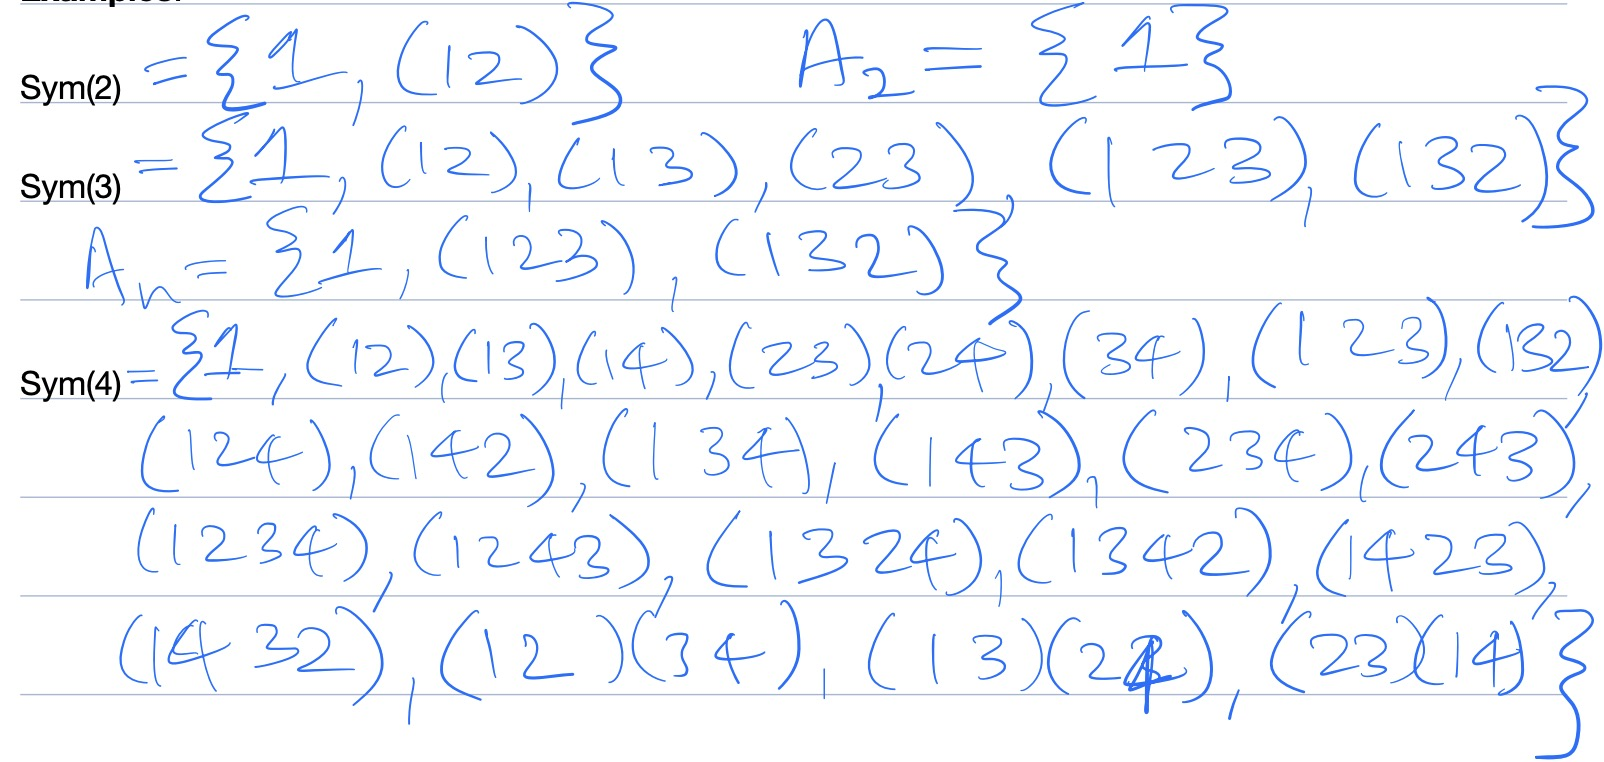
\includegraphics[width=1.0\textwidth]{Graphs/Alternative_Group.jpg} % 插入图片,并设置图片宽度为文本宽度的80%
    \end{figure}

\end{itemize}


\end{document}
